\documentclass{article}
\usepackage[margin=2cm]{geometry}
\usepackage{tabularx}
\usepackage{booktabs}
\usepackage{multirow}
\usepackage{enumitem}
\usepackage{url}
\usepackage{graphicx}
\usepackage{caption}
\usepackage{wrapfig}
\usepackage{setspace}
\usepackage{xcolor}
\usepackage{amsmath}
\usepackage{svg}



\makeatletter
\renewcommand{\maketitle}{\bgroup\setlength{\parindent}{0pt}
\begin{center} % Center the title
  \Large\@title
  \newline
  \footnotesize\@author
\end{center}
\begin{flushright}
  \@date
\end{flushright}
\egroup}
\makeatother

% Adjust line spacing
\setstretch{0.9}

% Adjust paragraph spacing
\setlength{\parskip}{0pt}

\begin{document}
\title{Impact of Liquidity Pool Size on Trading Volume in BTC-ETH Pools}
\author{
  Team \#111 \\
   \scriptsize Matias Vizcaino (avizcaino3) | Walter Jack Simmons (wsimmons35) | MingShen Wang (mwang709) | Vítor de Matos Castilho (vcastilho3)
}
\date{09 July 2023}
\maketitle



\noindent
{\setlength{\tabcolsep}{4pt} % Reduce column spacing

\section*{\textbf{Problem Statement and Objective}}

Decentralized Finance (DeFi), hosting about 48.78 billion USD in total value (as of April 23, 2023\footnote{\textit{"DefiLlama"} (2023), \url{https://defillama.com/}}), relies heavily on liquidity pools in decentralized exchanges like Uniswap for efficient crypto trading. These pools, using an automated market maker model, earn from trading fees distributed among liquidity providers based on their pool share.

This study primarily \textbf{aims to examine the influence of pool size on trading volume, specifically in BTC-ETH liquidity pools in exchanges like Uniswap}. It hypothesizes a direct correlation between pool size and trading volume, supported by existing studies. 

This understanding could optimize liquidity provision, enhance DeFi market efficiency, and benefit stakeholders. For instance, liquidity providers could improve fee returns and risk management, traders could refine strategies, and DeFi platforms could develop more effective liquidity pools.

\section*{\textbf{Uniswap Liquidity Pools: An Overview}}

Various DeFi platforms cater to different needs. Uniswap, a popular choice, provides a user-friendly interface and a broad spectrum of token pairs. Other platforms like Curve Finance and Balancer offer low-slippage trades and customizable pools, respectively.

Uniswap, a decentralized exchange (DEX) on Ethereum, supports trading of Ethereum-native and wrapped non-native assets. It uses a Constant Product Market Maker (CPMM) model in which liquidity providers deposit two tokens, keeping a constant product of reserves.

The CPMM formula is given by:

\[x \cdot y = k \quad \text{and} \quad price = \frac{y}{x}\]

Here, \(x\) and \(y\) denote the quantities of Token X and Y in the pool, and \(k\) is the constant product.

Uniswap operates without a central authority, ensuring privacy, fund control, and a diverse range of tokens. Centralized exchanges (CEX), though offering faster transaction speeds and better customer support, may pose security risks as they hold user funds.

Liquidity pools in DEXs enable direct interaction with smart contracts, ensuring continuous liquidity but exposing liquidity providers to impermanent loss risks. Prices are influenced by trade size, market conditions, supply-demand dynamics, and external price changes. Swaps and liquidity provision events, such as token minting and burning, significantly impact trading volumes. Indirect effects from network correlations and arbitrage opportunities can also influence trading volumes across pools.

\section*{\textbf{Introduction to Techniques Used to Solve the Problem}}

To address the problem statement and achieve our objectives, we will employ various techniques in our analysis. These techniques are commonly used in data analytics and quantitative research to explore relationships, make predictions, and gain insights from complex datasets. In this section, we provide an overview of the key techniques we will utilize in our study.

\subsection*{Regression Analysis}

Regression analysis is a widely used statistical technique for examining the relationship between a dependent variable and one or more independent variables. In our study, we will employ regression models, specifically Ordinary Least Squares (OLS) regression, to investigate the impact of liquidity pool size on trading volume. OLS regression allows us to estimate the coefficients of the independent variables and assess their significance in explaining the variation in the dependent variable.

\subsection*{Feature Engineering}

Feature engineering is the process of creating new features from existing data to improve the performance of machine learning models. In our analysis, we will perform feature engineering to construct additional variables that capture relevant information about liquidity pool dynamics, spillover effects, and price divergences. These engineered features will enhance the predictive power of our models and enable us to uncover meaningful patterns and relationships in the data.

\subsection*{Exploratory Data Analysis}

Exploratory Data Analysis (EDA) is an essential step in understanding and summarizing the main characteristics of a dataset. We will conduct EDA to generate descriptive statistics, visualizations, and correlation analyses. EDA will help us identify trends, outliers, and relationships between variables, providing valuable insights into the behavior of liquidity pool size and trading volume in BTC-ETH pools.

\subsection*{Model Evaluation and Optimization}

Model evaluation and optimization are crucial steps in developing accurate and robust predictive models. We will evaluate the performance of our regression models using metrics such as R-squared, which measures the proportion of variance in the dependent variable explained by the independent variables. Through model optimization, we will refine our feature selection, address multicollinearity, and explore alternative functional forms to improve the accuracy and interpretability of the models.

These techniques, along with our structured methodology, will enable us to analyze the relationship between liquidity pool size and trading volume in BTC-ETH pools effectively. By leveraging these techniques, we aim to provide valuable insights and recommendations to enhance liquidity provision, optimize trading strategies, and improve the efficiency of DeFi marketplaces.




\section*{Approach and Progress}
Overall, significant progress has been made in each stage of our approach. However, further analysis, evaluation, and optimization are required to successfully complete the project.

Throughout this process, we aim to maintain rigorous documentation of our methodologies and findings, which will allow us to ensure the transparency and replicability of our research.

\begin{table}[htbp]
\centering
\small
\begin{tabularx}{\linewidth}{|>{\raggedright\arraybackslash}X|}
\hline
\textbf{Data Collection:} Sourced data from multiple APIs (Uniswap, Binance) for liquidity pool sizes, trading volumes, and relevant variables. Data has been associated with Ethereum block numbers for consistent time measurement. Despite API rate limits, most of the data has been collected successfully. \\
\hline
\textbf{Data Preprocessing:} Cleaned, formatted, and addressed missing values in the dataset. Data consistency ensured and discrepancies from multiple sources addressed. Preprocessing completed with further examination of missing values in independent variables. Records with null values temporarily removed for continued analysis. \\
\hline
\textbf{Feature Engineering:} Constructed features to capture historical patterns, spillover effects, and price divergences utilizing a block-based time-series analysis framework. Feature engineering mostly complete, handling most direct pool features with finite lag. A review is planned to reduce the number of null values, include other feature categories, and perform feature selection. \\
\hline
\textbf{Exploratory Data Analysis:} Generated descriptive statistics, visualizations, and performed correlation analyses to uncover patterns, trends, and relationships between variables. In-depth exploratory data analysis will be performed once all features have been engineered, with various correlations and trends identified among the variables. \\
\hline
\textbf{Model Selection and Development:} Implemented a multivariate regression model (OLS) to investigate the pool size-trading volume relationship. Predicted target variables at different horizons with the application of lagged variables. OLS regression models have been developed and tested. Additional model testing and optimization in progress. \\
\hline
\textbf{Model Evaluation and Optimization:} Models evaluated using R-squared metric. Initial analyses indicate that model performance can be enhanced through further feature engineering/selection and reducing multicollinearity. Conducting correlation analysis and Variance Inflation Factor (VIF) for the final features. \\
\hline
\textbf{Final Analysis and Conclusions:} In the final stages of analysis. Commencing with drawing conclusions and communicating findings. Preparing to provide quantitative-driven insights. \\
\hline
\end{tabularx}
\caption{Approach and Progress}
\label{fig:approach-progress}
\end{table}



\vspace{-2em} % Reduce vertical spacing here
\section*{Challenges and Insights}

Data collection and processing required significant effort due to the advanced engineering involved. Notably, we faced challenges with the rate limits of the Etherscan free-tier API when gathering data via Python API calls.

We've adopted two time concepts to analyze liquidity pool dynamics\footnote{\textit{"DeFi: modeling and forecasting trading volume on Uniswap v3 liquidity pools"} (2023), \url{https://ssrn.com/abstract=444535}}. The "trading clock", defined by a block containing a mint operation, captures data temporal dynamics. A "time horizon" concept was introduced, defined every ten blocks up to the next mint operation, providing insights into the predictive power of independent variables over different timeframes.

Combined, these concepts allow a comprehensive exploration of short and long-term trends, informing decision-making and risk management in the DeFi ecosystem. Considering Uniswap operates on the Ethereum blockchain with a 14 seconds block time, these insights are invaluable.

The complexities of liquidity pool mathematics\footnote{\textit{"Liquidity Math in Uniswap V3"} (2021), \url{https://atiselsts.github.io/pdfs/uniswap-v3-liquidity-math.pdf}}\footnote{\textit{"A Primer on Uniswap v3 Math: As Easy As 1, 2, v3"} (2023), \url{https://blog.uniswap.org/uniswap-v3-math-primer}} presented hurdles, but we've captured the formulas to our best understanding in calculations.py functions. Given more time, we aim to refine these for enhanced feature derivation.



\section*{Dataset}

Inspired by the \textit{"DeFi modeling and forecasting trading volume" (2023)}\footnote{\textit{"DeFi: modeling and forecasting trading volume on Uniswap v3 liquidity pools"} (2023), \url{https://ssrn.com/abstract=444535}} paper, we sourced and constructed trade information for at least 6 months\footnote{\textit{Data Extracted and Cleansed}, \url{https://drive.google.com/drive/folders/1y5ZwLZK9GQYsCNYSY--4VQMg80dnuwuU?usp=sharing}}. Initial extraction work has already been performed, and you can refer to our GitHub repository\footnote{GitHub repository: \url{https://github.gatech.edu/MGT-6203-Summer-2023-Canvas/Team-111/tree/main/Code}} for further details and access to the code. The dataset consists of data obtained from the following sources:

\begin{center}
\small
\begin{tabular}{|p{0.15\linewidth}|p{0.35\linewidth}|p{0.5\linewidth}|}
\hline
\textbf{Source} & \textbf{Description} & \textbf{Data} \\
\hline
Uniswap's The Graph API\footnote{Uniswap's The Graph API: \url{https://api.thegraph.com/subgraphs/name/uniswap/uniswap-v3}} & Provides transaction details, trading volumes, and block information from Uniswap v3 liquidity pools. & Transaction IDs, timestamps, amounts, USD equivalents, and other related data. \\
\hline
Etherscan API\footnote{Etherscan API: \url{https://api.etherscan.io/api}} for Uniswap transaction hashes & Used to extract corresponding transaction data from Etherscan based on transaction hashes. & Block hashes, block numbers, sender addresses, gas details, transaction hashes, and other relevant information. \\
\hline
Binance\footnote{Binance GitHub Repository: \url{https://github.com/binance/binance-public-data/blob/master/python/README.md}} CEX Data for ETHBTC & Daily zip trades downloaded using provided scripts from the Binance GitHub repository. & Detailed information about each trade executed on the Binance platform, including trade prices, quantities, timestamps, and buyer/seller characteristics. \\
\hline
\end{tabular}
\end{center}


\section*{Key Variables}
\textbf{Target Variable:} Liquidity pool trading volumes (amountUSD) over specific blocks. We consider different models for multiple time horizons to study the relationship change over time.

\textbf{Independent Variables:}
The dependent variables are derived from a set of features and are categorized as follows [Mostly completed, refer to progress section]:
\begin{enumerate}[label=\arabic*. ,itemsep=0pt, topsep=0pt]
\item Direct pool features (41): volatility, rate, number of trades, average trade size.
\item CEX spillover effects (6): actual coin trade volume.
\end{enumerate}

We will aim to include as many variables as possible, given the time constraints of our project.




\section*{\textbf{In-Depth: Data and Feature Engineering}}

Feature engineering plays a crucial role in capturing the dynamics and relationships between variables in our analysis. The focus lies on engineering features that capture historical patterns of the DEX pools and spillover effects from CEX activity.

To start with, we can first define all the blocks in scope, then move to define the Reference blocks, and finally, the interval between reference blocks (which will be all the blocks in the interval).

Let's assume $B$ is the entire sequence of blocks within the scope of analysis and $K$ is the total number of blocks under study. We can represent this in the following way:

\begin{equation}
B = {b_k}_{k=1}^{K} \text{ where each } b_k \text{ is a block within the scope of analysis}
\end{equation}

In the construction of a time-series data model, the "Reference Block" acts as a chronological reference point. These blocks are key markers within the blockchain, identified based on Mint Operations when users provide liquidity to different pools on the decentralized exchange (DEX), such as Uniswap. The Reference Blocks are categorized into "same" and "other" pools. We position the most recent at the top and with an index of 0, so the sequence of blocks is ordered in decreasing chronological order.

\begin{equation}
R_{s} = \{b_{s}\}_{s=1}^{S} \text{ where each } b{s} \in B \text{ and is a reference block in the "same" pool}
\end{equation}

\begin{equation}
R_{o} = \{b_{o}\}_{o=1}^{O} \text{ where each } b{o} \in B \text{ and is a reference block in the "other" pool}
\end{equation}

Here, $S$ and $O$ are the total number of reference blocks in the "same" and "other" pools respectively.

Finally, the intervals between these reference blocks, which contain all blocks between $b_i$ and $b_j$ (inclusive of $b_i$), can be defined as the sequence of block numbers between $b_i$ and $b_j$. This can be expressed as:

\begin{equation}
I = {b_{ij}}_{\substack{i=0,j=i+1 \ i,j\leq N}}^N
\end{equation}

In this formula, $b_{ij}$ represents the sequence of blocks from $b_i$ to $b_{j-1}$, inclusive of $b_i$ and exclusive of $b_j$. This correctly captures the notion of an interval being all blocks "between" $b_i$ and $b_j$ in the blockchain sequence.


Block Reference Interval chains for the "same" and "other" pools' mint operations generate sequences of block numbers. These chains include the last N reference blocks and every block in between, where N signifies the number of lags or intervals analyzed for the direct features. Let $C_{s}$ and $C_{o}$ be the chains of "same" and "other" pools, which can be mathematically defined as:
\begin{equation}
  C = \{b_{i}\}_{i=0}^{N} \text{ where each } b{i} \text{ is a block} \in {R_s, R_o} \text{ and } b_{i} > b_{i+1} \text{ for } i \in {0,1,...,N-1}
  \end{equation}

Time horizons, representing future periods or timeframes for predictions or analyses of target variables, are constructed by starting from the first Reference Block and increasing the block count by M until the next reference block is reached. 
\begin{equation}
  H_{M} = \{b_{0}+kM\}_{k=0}^{K} \text{ with } K = \min \left( K_{max}, \left\lfloor \frac{\text{distance to next reference block}}{M} \right\rfloor \right)
  \end{equation}

  \begin{figure}[htbp]
    \begin{minipage}{0.5\textwidth}
      \centering
      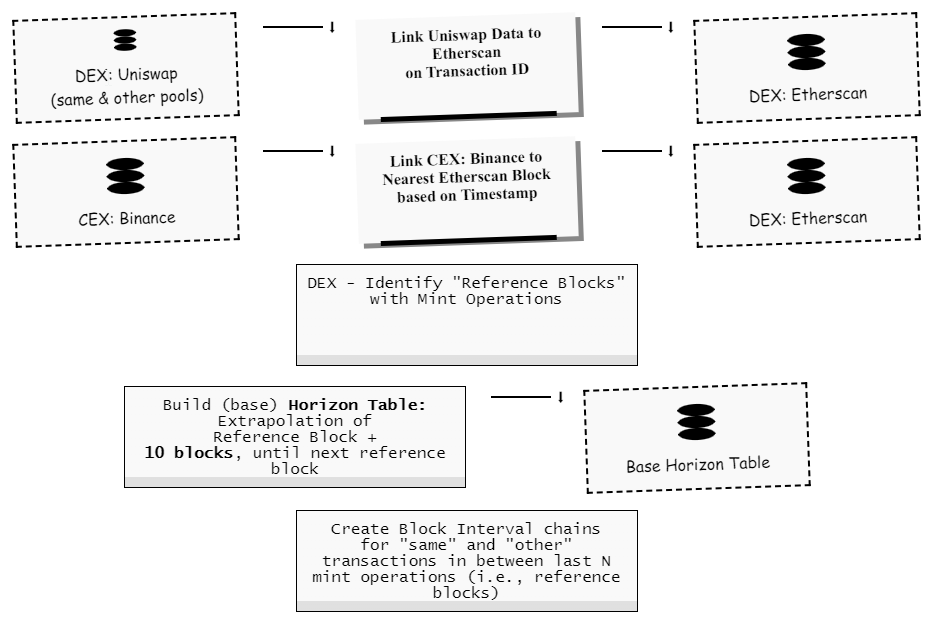
\includegraphics[width=\linewidth]{C:/Users/MatiasVizcaino/repos/6203-DataAnalyticsBusiness-Project/Other Resources/data-diagram/engineer.png}
      \caption{Data Engineering}
      \label{fig:data-diagram-engineer}
    \end{minipage}
    \begin{minipage}{0.45\textwidth}
      \centering
      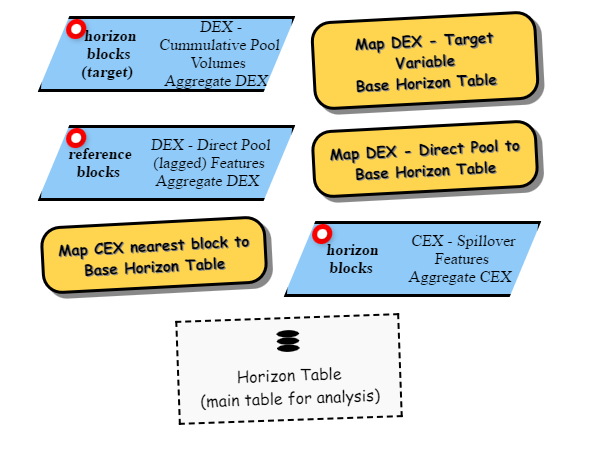
\includegraphics[width=\linewidth]{C:/Users/MatiasVizcaino/repos/6203-DataAnalyticsBusiness-Project/Other Resources/data-diagram/features.png}
      \caption{Feature Engineering}
      \label{fig:data-diagram-features}
    \end{minipage}
  \end{figure}

The Horizon Block Table captures the dynamics and relationships between the same/other/both pools by evaluating their respective target variables and features at different horizons and lags. The granularity level varies for each component within the Horizon Block Table, as illustrated in the following table:

\begin{equation}
  HBT = \{ (H_{M}, F_{DEX}, F_{DP}, F_{CEX}) \} \text{ for each horizon } H_{M} 
  \end{equation}
  

\begin{table}[htbp]
  \centering
  \begin{tabular}{|c|c|}
  \hline
  \textbf{Component} & \textbf{Granularity Level} \\
  \hline
  DEX target variable & Horizon block level \\
  \hline
  DEX direct pool features & Reference block level \\
  \hline
  CEX spillover features & Horizon block level \\
  \hline
  \end{tabular}
  \caption{Granularity Level of Components in Horizon Block Table}
  \label{table:granularity}
\end{table}

This granularity distinction allows for comprehensive examination of the behavior and interactions of the "same" and "other" pools at different levels within the time-series data model. The Horizon Block Table provides insights into the dynamics of the analyzed data, revealing the collaborative or competitive dynamics between the "same" and "other" pools throughout the time series.

\subsection*{Data Profiling: Highlights}

In terms of merging Uniswap transactions (txt) with Etherscan, we've observed a high match rate of transactions for the analysis period of six months. The transaction breakdown is as follows:

\begin{itemize}[leftmargin=*,noitemsep,nolistsep]
\small
\item Uniswap txs: ((500, 'burns'), 4000), ((500, 'mints'), 3406), ((500, 'swaps'), 217821), ((3000, 'burns'), 5918), ((3000, 'mints'), 5046), ((3000, 'swaps'), 48592)
\item Etherscan txs: ((500, 'burns'), 4000), ((500, 'mints'), 3242), ((500, 'swaps'), 217821), ((3000, 'burns'), 5918), ((3000, 'mints'), 4986), ((3000, 'swaps'), 48592)
\end{itemize}

From the transaction data, we created 8,227 reference blocks that correspond to each mint operation, excluding one. These blocks were then used to engineer features to calculate metrics for the same pool and other pools. These features capture data about liquidity pools and calculate metrics such as volatility, traded volume rate, trades count, and average volume. To expand the analysis, we have also included lagged features for the previous three mint operations. Table \ref{tab:chains} serves as our block reference table.

Before initiating the modeling phase, we need to address records with missing values in the independent variables. Notably, some null values have been identified in the volatility (same pool) and avg-USD/rate-USD (other pool) metrics. We have opted to remove these records temporarily to proceed with the analysis, with plans to reassess the calculations and mitigate the occurrence of null values likely resulting from lagged variables.

\begin{table}[htbp]
  \centering
  \small
  \begin{tabularx}{\linewidth}{|X|r|l|l|}
    \hline
    \textbf{pool} & \textbf{blockNumber} & \textbf{blockNumberChain} & \textbf{other\_blockNumberChain} \\
    \hline
    500 & 14498564 & [14498564, nan, nan, nan] & [14498564, nan, nan, nan] \\
    500 & 14498699 & [14498699, 14498564, nan, nan] & [14498699, nan, nan, nan] \\
    500 & 14499597 & [14499597, 14498699, 14498564, nan] & [14499597, 14499560, 14499457, 14499198] \\
    500 & 14499836 & [14499836, 14499597, 14498699, 14498564] & [14499836, 14499560, 14499457, 14499198] \\
    500 & 14500355 & [14500355, 14499836, 14499597, 14498699] & [14500355, 14500043, 14499560, 14499457] \\
    ... & ... & ... & ... \\
    3000 & 15648981 & [15648981, 15648330, 15648305, 15648187] & [15648981, 15648887, 15648536, 15646933] \\
    3000 & 15649246 & [15649246, 15648981, 15648330, 15648305] & [15649246, 15649243, 15648887, 15648536] \\
    3000 & 15649545 & [15649545, 15649246, 15648981, 15648330] & [15649545, 15649522, 15649347, 15649269] \\
    3000 & 15649565 & [15649565, 15649545, 15649246, 15648981] & [15649565, 15649522, 15649347, 15649269] \\
    3000 & 15649578 & [15649578, 15649565, 15649545, 15649246] & [15649578, 15649522, 15649347, 15649269] \\
    \hline
  \end{tabularx}
  \caption{BlockNumber Chains}
  \label{tab:chains}
\end{table}

Finally, we've constructed a base table \ref{tab:horizon} with the \texttt{start\_blockNumber} of each horizon and the \texttt{reference\_blockNumber}, defined by mint operations in the block. This base table is joined with the mint aggregated transaction data to generate our target variables and independent variables that are lagged.

\begin{table}[htbp]
  \centering
  \small
  \begin{tabular}{cccccc}
    \hline
    \textbf{blockNumber} & \textbf{min\_flag} & \textbf{reference\_blockNumber} & \textbf{horizon\_label} & \textbf{cum\_volume\_500} \\
    \hline
    108757 & 0 & 15552674 & 9 & 423485.346309 \\
    108758 & 0 & 15552674 & 10 & 423485.346309 \\
    108759 & 1 & 15552772 & 1 & 328338.732259 \\
    108760 & 0 & 15552772 & 2 & 406084.780730 \\
    108761 & 0 & 15552772 & 3 & 536640.714920 \\
    ... & ... & ... & ... & ... \\
    109047 & 0 & 15555464 & 12 & 122730.731534 \\
    109048 & 0 & 15555464 & 13 & 123650.594764 \\

    \hline
  \end{tabular}
  \caption{Reference and Horizon blocksn}
  \label{tab:horizon}
\end{table}

\section*{\textbf{In-Depth: Modelling Techniques}}

In our analysis, we will employ regression models to investigate the relationship between liquidity pool size and trading volume. Specifically, we will use an Ordinary Least Squares (OLS) regression approach.

We will develop and test OLS regression models for different target variables and horizons. Lagged variables will be incorporated into the models to predict trading volumes at different time horizons. The performance of the models will be evaluated using metrics like R-squared.

Additional modelling techniques and considerations, such as addressing autocorrelation, endogeneity, structural breaks, and multicollinearity, will be applied to enhance the accuracy and interpretability of the models.


We have commenced the development of a framework for our prediction models and have constructed several Proof of Concept (PoC) models. For the modeling phase, we're employing an Ordinary Least Squares (OLS) regression approach to predict multiple target variables across different horizons using a set of independent lagged variables for each reference mint. This process involves iterating over the horizons, generating data subsets, fitting an OLS model for each horizon, and retrieving the R-squared value as a performance indicator. This approach allows for efficient and consistent prediction across various horizons.

\[
\text{{cum\_volume\_500}}_\text{{horizon}} = \beta_0 + \beta_1 \cdot \widetilde{01}X + \beta_2 \cdot \widetilde{12}X + \beta_3 \cdot \widetilde{23}X + \ldots + \epsilon
\]

In this formula, \(\beta_0\), \(\beta_1\), \(\beta_2\), \(\beta_3\), etc., represent the coefficients associated with each spot lagged variable, while \(\epsilon\) denotes the error term or residual.

\begin{wrapfigure}[16]{l}{0.35\textwidth}
\vspace{0pt} % Adjust the vertical spacing as needed
\centering
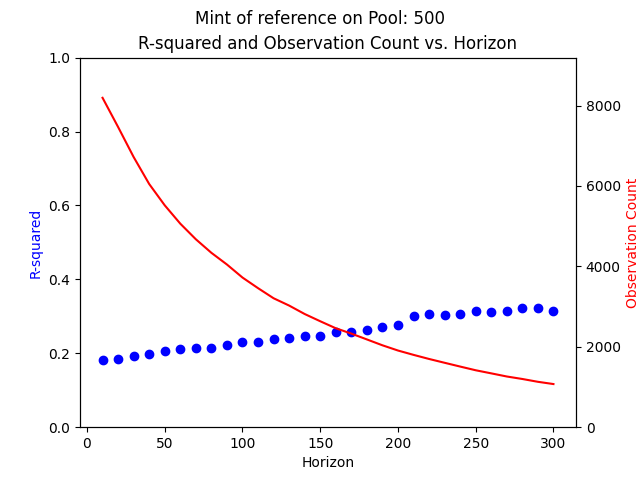
\includegraphics[width=\linewidth]{C:/Users/MatiasVizcaino/repos/6203-DataAnalyticsBusiness-Project/Other Resources/R2Horizon.png}
\caption{R2 best fit horizon}
\label{fig:R2-horizon}
\end{wrapfigure}

Observations indicate that around the horizon 20 (200 blocks, approximately 13 minutes), the R2 value ceases to increase significantly. Preliminary analysis of the relevant model (at horizon 20) reveals that the OLS regression model explains approximately 27.6\% of the variation in the dependent variable cum\_volume\_3000\_ref500. The significant variables, such as rate-count-isame\_01, rate-count-isame\_12, rate-count-isame\_23, and wlother\_3, have a considerable impact on the dependent variable. However, the potential collinearity among the independent variables could affect the interpretation of individual coefficients, suggesting a need for further analysis.

Model selection will be based on the optimal combination of features for each horizon. As we refine the feature and model development, considerations like autocorrelation, endogeneity, structural breaks, or multicollinearity will be addressed. These will be managed through additional sensitivity analyses, cross-validations, and the application of appropriate statistical techniques to diagnose and mitigate any complexities.


\section*{\textbf{Model Optimisation and Selection}}

Once the initial models are developed, we will evaluate their performance and optimize them for better accuracy and predictive power. Model optimization may involve refining the feature selection, reducing multicollinearity, and exploring alternative functional forms or transformations of variables.

Model selection will be based on the optimal combination of features, horizons, and target variables that provide accurate predictions and meaningful insights.

\section*{\textbf{Analysis and Discussion}}

In the final stages of our analysis, we will conduct an in-depth examination of the results and draw conclusions based on the findings. We will analyze the relationships between liquidity pool size and trading volume in BTC-ETH pools, considering other factors such as spillover effects and price divergences.

We will discuss the implications of our findings for liquidity provision, DeFi market efficiency, and various stakeholders. The quantitative-driven insights from our analysis can help optimize liquidity provision, refine trading strategies, and improve the effectiveness of liquidity pools in the DeFi ecosystem.

\end{document}


\section*{Going Forward}

To summarize, the learnings from this project, particularly regarding data engineering and feature generation, are substantial. This largely unexplored field of financial technology presents vast opportunities for fresh findings and contributions to the existing body of knowledge. Our initial results are promising, and we're eager to delve into the forthcoming phases of our project, emphasizing model optimization and refining our analysis and conclusions.

Our future steps in the modeling phase include:

\begin{itemize}
\item Dataset Splitting: Partitioning the dataset into training and test sets, performing model metrics analysis, and interpretation.
\item Analysis Scope: Examining both Pool 500 and Pool 3000, with a focus on target variables related to volume on the same pool as the reference mint, the other pool, or both.
\item Experimentation: Identifying the optimal combinations of features, horizons, and target variables for accurate predictions.
\item Feature Selection: Using techniques like step-wise or Principal Component Analysis to reduce feature complexity, limit overfitting, and improve interpretability.
\end{itemize}

Our planned experiments include testing different lag lengths, incorporating quadratic features or interaction terms, and accounting for structural breaks, such as the Terra-Luna collapse (May 2022) and the Merge (Sep 2022).

We aspire here or on further work to drive a comprehensive analysis and quantitative discussion on:

\begin{enumerate}[itemsep=0pt, topsep=0pt]
\item The relationship between liquidity pool size and trading volume in BTC-ETH liquidity pools.
\item The influence of the liquidity pool size on the slippage in BTC-ETH trading pairs, considering CEX spillover effects.
\item Impact of BTC-ETH price volatility on trading volume relative to liquidity pool size, focusing on price divergence.
\item Specific periods/events that significantly affect the relationship between BTC-ETH liquidity pool size and trading volume.
\end{enumerate}



\section*{\textbf{Future Extensions}}
Future extension:

Future extensions may include price divergences in BTC-ETH exchanges and pools, as arbitrage opportunities may also drive activity.

\begin{enumerate}[label=\arabic*. ,itemsep=0pt, topsep=0pt]
\item Direct pool features (2): total value locked (TVL)
\item Network spillover effects (8): trade flow imbalance.
\item Price divergences between the 500 and 3000 pools (2).
\end{enumerate}




\end{document}